\subsection{metaPCA}
Dimension reduction is a popular data mining approach for transcriptomic analysis.
MetaPCA aims to combine multiple omics datasets of identical or similar biological hypothesis and perform simultaneous dimensional reduction in all studies.
The results show improved accuracy, robustness and better interpretation among all studies.
By clicking toolsets and then metaPCA,
users are directed to metaPCA home page as Figure~\ref{fig:metaPCAHome}.

\begin{figure}[H]
\begin{center}
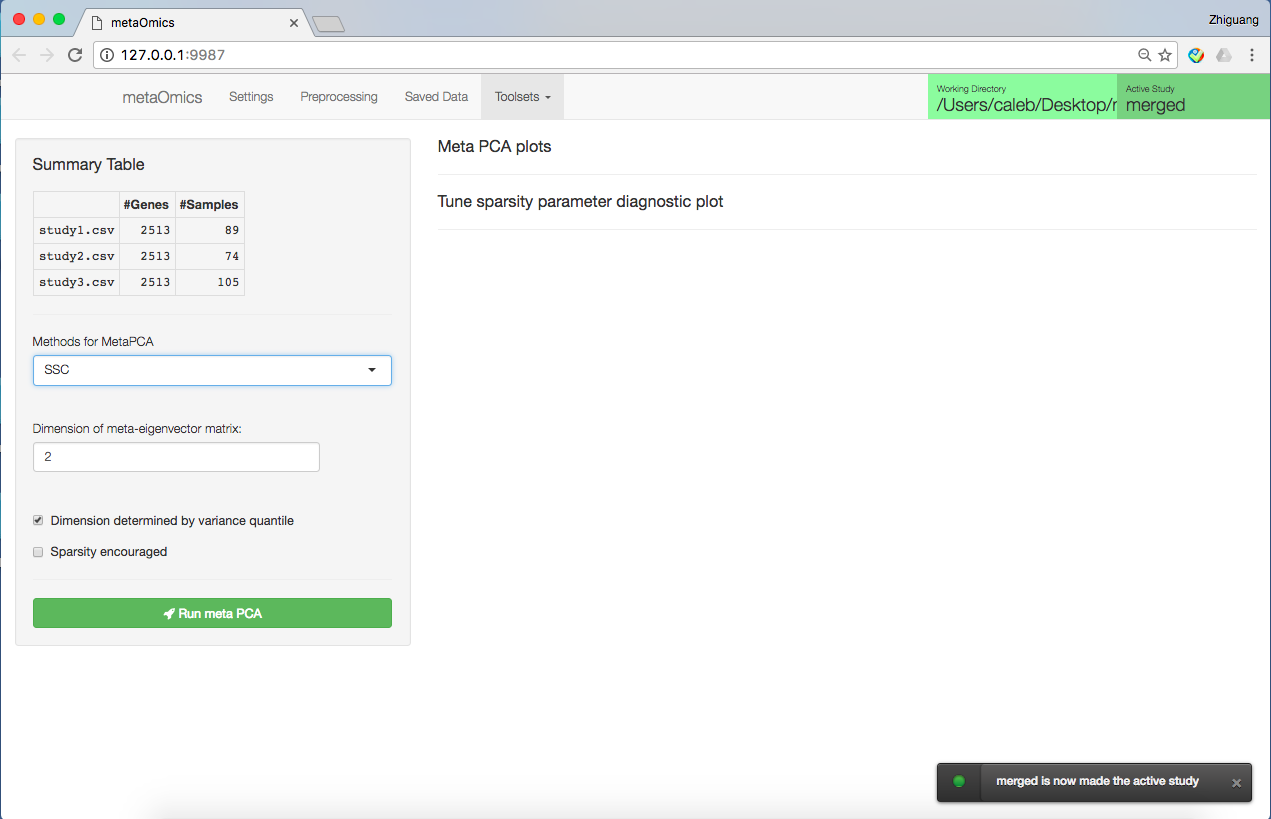
\includegraphics[scale=0.4]{./figure/metaPCA/metaPCAHome}
\caption{GUI Preprocessing page}
\label{fig:metaPCAHome}
\end{center}
\end{figure}

\subsubsection{Procedure}

\begin{steps}

\item \textbf{Specify parameters} 
There are very few parameter to be specify in metaPCA.

\end{steps}

\subsubsection{Methods for MetaPCA}

\begin{itemize}
\item MetaPCA via sum of variance decomposition (SV)

Let $X^{(m)}$ be an observed $p\times n^{(m)}$ data matrix of sample size $n^{(m)}$ and $p$ features for study $m$ 
($1 \leq m\leq M$). 
Denote by $S^{(m)}$ the maximum likelihood (ML) estimate of the $p \times p$ covariance matrix $\Omega^{(m)}$ of $X^{(m)}$. 
MetaPCA via sum of variance decomposition (SV) aims to solve the following eigen-value decomposition problem.
\begin{equation}\label{eq:eq2}
T^{SV}=\sum_{m=1}^M w^{(m)} S^{(m)},
\end{equation}
where $w^{(m)}$ is the reciprocal of the largest eigenvalue of $S^{(m)}$.
%{\color{red} (Do we need to explain scree plot here or later in SSC?} {\color{blue} SungHwan's answer: I believe either way should be fine. Here I add the scree plot strategy in the following section.)}
The common principal components $L$ are calculated from the eigen-decomposition of $T^{SV}: L^T(T^{SV})L = \Lambda$ and $K$ top common PCs should be retained for down-stream analysis. Selection of the optimal $K$ will be described later in the the section of Parameter selection. 

\item MetaPCA via sum of squared cosine (SSC) maximization.

the second MetaPCA framework motived by SSC criterion proceeds as below.
The top $j^{(m)}$ eigenvectors are calculated from study $m$ to form eigenvector matrix $V^{(m)}$.
We then perform eigen-decomposition on $T^{\mbox{SSC}} = \sum_{m=1}^M V^{(m)} V^{(m)^T}$ and select the top $K$ eigenvectors to form the meta-analytic common eigen-space:

\begin{equation}
\Big (\sum_{m=1}^M V^{(m)} V^{(m)^T} \Big ) B^{SSC} = \Lambda^* B^{SSC}
\end{equation}
where $V^{(m)}$ is a matrix consisting of $j^{(m)}$ leading eigenvectors,
$\Lambda^*$ is a diagonal eigenvalue matrix, and $B^{\mbox{SSC}} = (\beta_1^{\mbox{SSC}}, \dots, \beta_K^{\mbox{SSC}})$ contains the top $K$ eigenvectors.

\end{itemize}

\subsubsection{Dimension of meta-eigenvector matrix}
Dimension of meta-eigenvector matrix option allows user to specify dimension of the output meta-eigenvector matrix.

\subsubsection{Dimension determined by variance quantile}
Logical value whether dimension size of each study's eigenvector matrix (SSC) is determined  by the pre-defined level of variance quantile 80\%.

\subsubsection{Sparsity encouraged}
If the Sparsity encouraged checkbox is selected, 
we are able to tune the best tuning parameter $\lambda$ and perform sparse metaPCA.
After clicking on search for optimal tuning parameter button, the optimum tuning parameter will be returned to the box ``tuning parameter for sparsity"

\subsubsection{Run meta PCA}
If Sparsity encouraged checkbox is selected, sparse meta PCA will be performed. 
Otherwise, meta PCA will be performed.
The result is shown in the following figures.

\begin{figure}[H]
\begin{center}
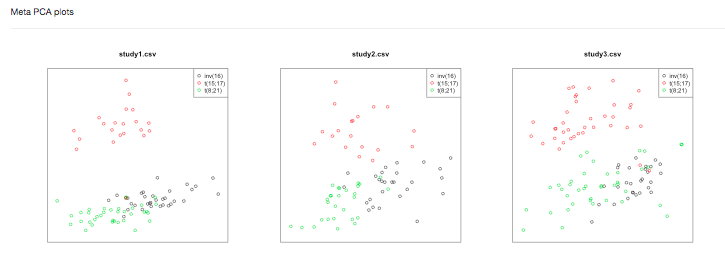
\includegraphics[scale=0.4]{./figure/metaPCA/metaPCA}
\caption{GUI Preprocessing page}
\label{fig:metaPCAresult}
\end{center}
\end{figure}

